% !TEX program = xelatex
\documentclass[11pt]{article}

\usepackage[margin=0.86in,headheight=22pt]{geometry}
\usepackage{fontspec}
\setmainfont{Charter}
\setsansfont{Avenir Next}
\setmonofont[Scale=0.88]{Menlo}
\usepackage{microtype}
\usepackage{setspace}
\setstretch{1.055}
\usepackage{amsmath,amssymb,mathtools}
\usepackage{booktabs,tabularx,array,multirow}
\usepackage{graphicx}
\usepackage[dvipsnames]{xcolor}
\usepackage{tikz}
\usetikzlibrary{arrows.meta,positioning,fit,calc,shapes.geometric,backgrounds}
\usepackage[most]{tcolorbox}
\usepackage{enumitem}
\usepackage{titlesec}
\usepackage{fancyhdr}
\usepackage{caption}
\usepackage{hyperref}
\usepackage{xurl}
\usepackage{lastpage}

\definecolor{DmonInk}{HTML}{17212B}
\definecolor{DmonBlue}{HTML}{235789}
\definecolor{DmonCyan}{HTML}{2C8C99}
\definecolor{DmonGreen}{HTML}{3A7D44}
\definecolor{DmonGold}{HTML}{B67A1B}
\definecolor{DmonRed}{HTML}{A33A3A}
\definecolor{DmonPale}{HTML}{F3F6F8}
\definecolor{DmonRule}{HTML}{CBD5DE}

\hypersetup{
  colorlinks=true,
  linkcolor=DmonBlue,
  citecolor=DmonGreen,
  urlcolor=DmonBlue,
  pdftitle={DMON-1: Toward a Persistent, Growing Neural Organism},
  pdfauthor={DMON-1 Research Project},
  pdfsubject={Working research report on the SOL2 organism and detachable cognitive organs}
}

\pagestyle{fancy}
\fancyhf{}
\lhead{\sffamily\small DMON-1 Research Report}
\rhead{\sffamily\small Persistent Neural Organisms}
\cfoot{\sffamily\small \thepage\ / \pageref*{LastPage}}
\renewcommand{\headrulewidth}{0.35pt}
\renewcommand{\headrule}{\hbox to\headwidth{\color{DmonRule}\leaders\hrule height \headrulewidth\hfill}}

\titleformat{\section}
  {\sffamily\Large\bfseries\color{DmonInk}}{\thesection}{0.7em}{}
\titleformat{\subsection}
  {\sffamily\large\bfseries\color{DmonBlue}}{\thesubsection}{0.65em}{}
\titleformat{\subsubsection}
  {\sffamily\normalsize\bfseries\color{DmonInk}}{\thesubsubsection}{0.6em}{}
\titlespacing*{\section}{0pt}{2.2ex plus .4ex}{1.1ex}
\titlespacing*{\subsection}{0pt}{1.8ex plus .3ex}{0.8ex}

\makeatletter
\renewcommand*\l@section{\@dottedtocline{1}{0em}{2.6em}}
\makeatother

\setlist[itemize]{leftmargin=1.45em,itemsep=0.28em,topsep=0.35em}
\setlist[enumerate]{leftmargin=1.6em,itemsep=0.28em,topsep=0.35em}
\captionsetup{font=small,labelfont={bf,sf},textfont=it}
\renewcommand{\arraystretch}{1.16}

\newcommand{\dmon}{\textsf{DMON-1}}
\newcommand{\soltwo}{\textsf{SOL2}}
\newcommand{\bpc}{\textsf{BPC}}
\newcommand{\established}{\textcolor{DmonGreen}{\textbf{Established}}}
\newcommand{\mechanistic}{\textcolor{DmonBlue}{\textbf{Mechanistic evidence}}}
\newcommand{\diagnostic}{\textcolor{DmonGold}{\textbf{Diagnostic}}}
\newcommand{\openclaim}{\textcolor{DmonRed}{\textbf{Open}}}

\newtcolorbox{claimbox}[1]{
  enhanced, breakable,
  colback=DmonPale,
  colframe=DmonBlue,
  boxrule=0.6pt,
  arc=2pt,
  left=7pt,right=7pt,top=6pt,bottom=6pt,
  title={#1},
  coltitle=white,
  colbacktitle=DmonBlue,
  fonttitle=\sffamily\bfseries
}

\newtcolorbox{warningbox}[1]{
  enhanced, breakable,
  colback=white,
  colframe=DmonGold,
  boxrule=0.7pt,
  arc=2pt,
  left=7pt,right=7pt,top=6pt,bottom=6pt,
  title={#1},
  coltitle=DmonInk,
  colbacktitle=DmonGold!18,
  fonttitle=\sffamily\bfseries
}

\begin{document}

\begin{titlepage}
  \pagecolor{DmonPale}
  \color{DmonInk}
  \vspace*{1.0cm}
  {\sffamily\Large DMON-1 Research Project\par}
  \vspace{1.4cm}
  {\sffamily\bfseries\fontsize{32}{37}\selectfont
    Toward a Persistent,\\[0.18em]
    Growing Neural Organism\par}
  \vspace{0.65cm}
  {\sffamily\Large
    Typed cellular computation, detachable cognitive organs,\\
    continual adaptation, and frozen-LLM language control\par}

  \vfill

  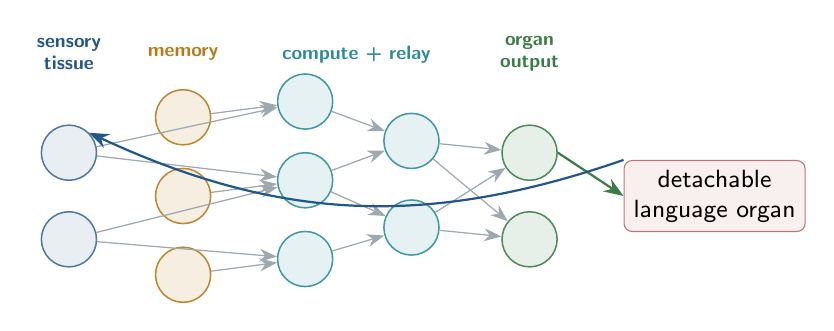
\begin{tikzpicture}[x=1cm,y=1cm]
    \tikzset{
      cell/.style={circle, minimum size=7mm, inner sep=0pt, draw=DmonBlue!80,
        fill=DmonBlue!10, line width=.55pt},
      memory/.style={cell,draw=DmonGold!90,fill=DmonGold!13},
      relay/.style={cell,draw=DmonCyan!90,fill=DmonCyan!12},
      output/.style={cell,draw=DmonGreen!90,fill=DmonGreen!12},
      edge/.style={-{Stealth[length=2.2mm]},draw=DmonRule!75!DmonInk,line width=.45pt}
    }
    \node[cell] (i1) at (0,1.1) {};
    \node[cell] (i2) at (0,0) {};
    \node[memory] (m1) at (1.45,1.55) {};
    \node[memory] (m2) at (1.45,.55) {};
    \node[memory] (m3) at (1.45,-.45) {};
    \node[relay] (c1) at (3.0,1.75) {};
    \node[relay] (c2) at (3.0,.75) {};
    \node[relay] (c3) at (3.0,-.25) {};
    \node[relay] (c4) at (4.35,1.25) {};
    \node[relay] (c5) at (4.35,.15) {};
    \node[output] (o1) at (5.85,1.1) {};
    \node[output] (o2) at (5.85,0) {};
    \foreach \a/\b in {i1/c1,i1/c2,i2/c2,i2/c3,m1/c1,m2/c2,m3/c3,c1/c4,c2/c4,c2/c5,c3/c5,c4/o1,c4/o2,c5/o1,c5/o2}
      \draw[edge] (\a) -- (\b);
    \node[anchor=center,font=\sffamily\scriptsize\bfseries,align=center,text=DmonBlue]
      at (0,2.35) {sensory\\tissue};
    \node[anchor=center,font=\sffamily\scriptsize\bfseries,text=DmonGold]
      at (1.45,2.35) {memory};
    \node[anchor=center,font=\sffamily\scriptsize\bfseries,text=DmonCyan]
      at (3.65,2.35) {compute + relay};
    \node[anchor=center,font=\sffamily\scriptsize\bfseries,align=center,text=DmonGreen]
      at (5.85,2.35) {organ\\output};
    \node[draw=DmonRed!70,fill=DmonRed!8,rounded corners=3pt,minimum width=2.3cm,
      minimum height=.85cm,font=\sffamily\small,align=center] (llm) at (8.2,.55)
      {detachable\\language organ};
    \draw[-{Stealth[length=2.5mm]},draw=DmonGreen,line width=.8pt] (o1.east) -- (llm.west);
    \draw[-{Stealth[length=2.5mm]},draw=DmonBlue,line width=.8pt,bend left=22]
      (llm.north west) to (i1.north east);
  \end{tikzpicture}

  \vfill
  {\sffamily\large Working research report\par}
  \vspace{0.15cm}
  {\sffamily\normalsize 4 August 2026\par}
  \vspace{0.7cm}
  {\small
  This document reports implemented systems and completed experiments through
  \textsf{L0-C1g}. Claims are labeled by evidential status; exploratory results are
  not promoted into capability claims.\par}
\end{titlepage}
\nopagecolor

\begin{abstract}
\noindent
\dmon{} is an attempt to build a persistent neural creature rather than a stateless
task model: a continuously stimulated cellular network whose internal state, learned
anatomy, developmental history, and detachable organs together constitute the agent.
The current implementation, \soltwo{}, uses typed neural tissues on a sparse directed
connectome, bounded recurrent operators, private cell expression and low-rank private
transitions, stream-written memory, dedicated output tissue, append-only growth, and
complete living-state checkpoints. Language is treated as a replaceable organ. A frozen
Llama-3 8B model supplies contextual sensory features and fluent decoding, while the
organism alone owns new trainable state and emits bounded low-rank controls.

The program has established several mechanistic results. Cellular recurrent state is
causal for character prediction; bounded typed tissue yields replicated dependence on
cell identity and learned topology; a mastered organism accelerates acquisition through
a newly attached organ; removed organs can be reattached and rapidly recovered; utility
anchors substantially improve the stability--plasticity frontier; and a frozen 8B
language model can be integrated with exact zero-control parity and zero backbone
gradients. The program has not yet established simultaneous mastery of multiple deep
procedures, useful recruitment of pressure-grown neurons, autonomous conversation, or
held-out factual recall through the organism. The latest memory experiments localize a
real signal from retained memory through internal tissue, but show collapse at output
tissue and insufficient training of the LLM-control geometry. These results support the
feasibility of the organism concept while sharply defining the remaining work.
\end{abstract}

\tableofcontents
\clearpage

\section{Research Objective}

The project asks whether an artificial neural system can be organized as a living,
developing substrate rather than as a fixed inference graph. The long-term target is a
small creature that can grow, remain continuously active, acquire new organs, integrate
new experience into a persistent internal world, and converse with a user. ``DMON'' is
an intentional contraction of ``Digimon'': the desired endpoint is not merely a better
benchmark model, but a recognizable individual with whom interaction is possible.

This changes the role of language modelling. A large language model is treated as
Broca-like machinery: a powerful organ for linguistic representation and production,
not the whole cognitive organism. The cellular substrate is intended to provide the
rest of the loop: lifetime memory, mode selection, cross-modal integration, adaptation,
development, motivation, and continuity of self. The design therefore does not aim to
beat a transformer or GRU on every small closed-world task. Those models remain useful
controls, but low bits-per-character alone cannot measure growth, lifelong plasticity,
or multi-organ integration.

\begin{claimbox}{Central feasibility question}
Can a persistent, locally connected neural organism develop useful internal structure,
retain and reuse computations while its interfaces change, add capacity without being
rebuilt, and control detachable pretrained organs without surrendering its identity to
those organs?
\end{claimbox}

The project deliberately distinguishes four levels of evidence:

\begin{itemize}
  \item \established{} means a software or numerical contract was directly verified,
        usually with matched controls and deterministic artifacts.
  \item \mechanistic{} means a causal intervention localized behavior to cellular state,
        tissue, topology, an organ, or newly introduced machinery.
  \item \diagnostic{} means an experiment usefully localized a bottleneck but did not
        satisfy the capability gate.
  \item \openclaim{} marks a project goal for which present evidence is insufficient.
\end{itemize}

\section{Design Commitments}

\subsection{The creature is the network}

Earlier work explored a visible morphology on a resource field. That work remains
useful as a future display organ, but it is not the central creature. In the current
architecture, the creature is the persistent neural network itself. Sensory modalities,
language, audio, and visible morphology are organs coupled to the same cellular state.
This distinction prevents a visually compelling body from being mistaken for the
computational organism.

\subsection{Persistent state and continual stimulation}

The organism does not conceptually begin and end with task episodes. Its state survives
tokens, optimizer boundaries, checkpoint/resume, organ removal, and organ reattachment.
Current result-bearing trainers still use finite truncated backpropagation windows;
therefore the implemented system should be described as a persistent stream learner,
not yet as a fully asynchronous biological learner. A separate versioned runtime keeps
foreground ticks and background optimization distinct, but the strict asynchronous
milestone remains open.

\subsection{Anatomy should matter, but lesions need not be tolerated}

Input, memory, compute, relay, and output tissue have different roles. Output cells are
sinks that read only compute and relay tissue, so a decoder cannot directly bypass the
body. Acute freeze, state-shuffle, identity-shuffle, and topology-rewire experiments are
used to identify what carries a learned capability. They are not adversarial conditions
the organism is expected to survive. In biological terms, destroying grey-matter state
or rewiring white-matter routes should damage the learned computation.

An important methodological correction emerged during the Fable experiments:
\emph{freezing} a population measures whether it does work, while \emph{shuffling}
within a tissue measures whether cell identity or placement is differentiated. Useful
mean-field tissue can be nearly shuffle-invariant. Reporting both avoids calling an
interchangeable population ``unused.''

\subsection{Reserve is permitted}

The project does not reward every neuron for being active. Some internal cells may be
dormant or weakly used, providing reserve for later plasticity. The relevant conditions
are that a nontrivial subset is causally useful, the active computation traverses the
organism, and claimed new tissue is actually recruited when growth is invoked.

\subsection{Information metabolism and satiety}

The intended economy is denominated in reducible information, not raw activity or raw
surprise. Paying for unpredictable input creates a noisy-TV optimum; paying for
prediction progress rewards structure that can be learned. Metabolism is currently
deferred from \soltwo{} until capability and continual credit assignment are sufficiently
understood. The eventual human loop also requires satiety: a creature rewarded without
bound for attention would be structurally encouraged to manipulate its user.

\section{The SOL2 Organism}

\subsection{Typed tissues on a sparse directed connectome}

\soltwo{} replaces the earlier accidental assumption of one universal cell rule with
one rule per tissue and bounded private expression per mutable cell. The current tissue
layout is:

\begin{itemize}
  \item \textbf{Input tissue.} Receives bounded organ-specific sensory drive and begins recurrent
        integration.
  \item \textbf{Stream-memory tissue.} Receives differentiable external writes through a finite
        FIFO; mutable cells cannot write it directly.
  \item \textbf{Compute tissue.} Performs recurrent transformation under its typed rule and
        private expression.
  \item \textbf{Relay tissue.} Supplies transport capacity, append-only growth, and an anatomical
        reserve that can connect old and new circuitry.
  \item \textbf{Output tissue.} Is cleared at token boundaries, receives only compute/relay input,
        and is read by the active output organ.
\end{itemize}

Each target cell owns a fixed number of dendrite slots. Installed slots name explicit
source cells; dormant slots carry exactly zero message and reserve anatomical capacity.
Attention is local to those named dendrites. Output cells are never sources and their
dendrites may not read input or memory tissue, which makes the no-bypass constraint
executable rather than rhetorical.

\begin{figure}[ht]
\centering
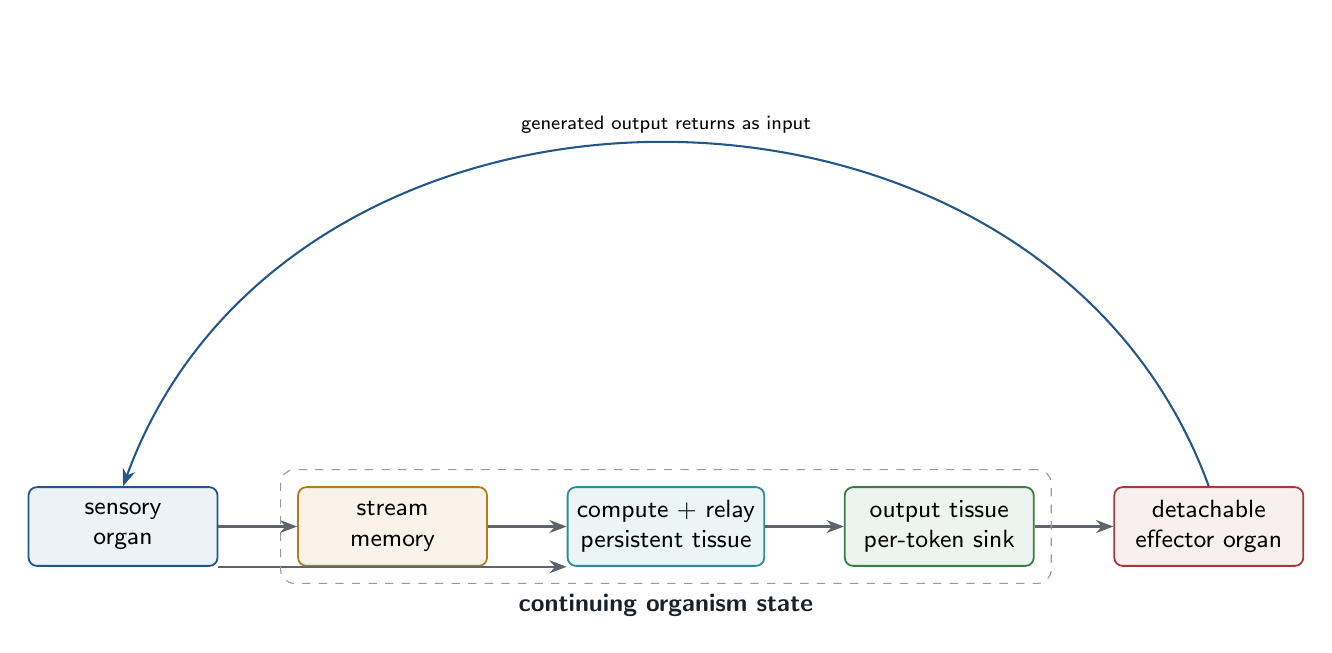
\begin{tikzpicture}[node distance=9mm and 10mm,>=Stealth]
  \tikzset{
    block/.style={draw,rounded corners=3pt,minimum height=10mm,minimum width=24mm,
      align=center,font=\sffamily\small,line width=.65pt},
    flow/.style={-{Stealth[length=2.2mm]},line width=.75pt,draw=DmonInk!70},
    feedback/.style={-{Stealth[length=2.2mm]},line width=.75pt,draw=DmonBlue}
  }
  \node[block,draw=DmonBlue,fill=DmonBlue!8] (sense) {sensory\\organ};
  \node[block,draw=DmonGold,fill=DmonGold!10,right=of sense] (memory) {stream\\memory};
  \node[block,draw=DmonCyan,fill=DmonCyan!9,right=of memory] (internal) {compute + relay\\persistent tissue};
  \node[block,draw=DmonGreen,fill=DmonGreen!9,right=of internal] (output) {output tissue\\per-token sink};
  \node[block,draw=DmonRed,fill=DmonRed!8,right=of output] (organ) {detachable\\effector organ};
  \draw[flow] (sense) -- (memory);
  \draw[flow] (sense.south east) -- (internal.south west);
  \draw[flow] (memory) -- (internal);
  \draw[flow] (internal) -- (output);
  \draw[flow] (output) -- (organ);
  \draw[feedback] (organ.north) to[out=110,in=70,looseness=1.15]
    node[above,font=\sffamily\scriptsize]{generated output returns as input} (sense.north);
  \node[draw=DmonInk!45,dashed,rounded corners=5pt,fit=(memory)(internal)(output),inner sep=6pt,
    label={[font=\sffamily\small\bfseries,text=DmonInk]below:continuing organism state}] {};
\end{tikzpicture}
\caption{The organism owns persistent state and recurrent anatomy. Sensory and effector
organs may be attached or removed; all behaviorally relevant control must traverse
compute/relay tissue and the dedicated output sink.}
\label{fig:architecture}
\end{figure}

\subsection{Bounded cellular dynamics}

For mutable cell $i$ at transition $t$, \soltwo{} combines current state $h_{i,t}$,
aggregated dendritic message $m_{i,t}$, and organ drive $d_{i,t}$. A typed tissue rule
produces a bounded target, optionally shifted by private expression $e_i$ and a private
low-rank residual $r_i$:

\begin{align}
  z_{i,t} &= f_{\tau(i)}\!\left([h_{i,t},m_{i,t},d_{i,t}]\right) + e_i + r_i,\\
  \alpha_{i,t} &\in [0.02,0.80],\\
  h_{i,t+1} &= (1-\alpha_{i,t})h_{i,t} + \alpha_{i,t}\tanh(z_{i,t}).
\end{align}

The bounded update keeps mutable state in $[-1,1]$ from a zero initial state. Private
target/time-constant expression gives cell identity without requiring a separate dense
network per cell. Later experiments add rank-four private transition residuals whose up
projection begins at zero, so the treatment is initially behaviorally silent and can be
recruited by gradient descent.

For target $i$ with installed sources $\mathcal{N}(i)$, the directed connectome uses
bounded query/key/value maps and a learned edge bias $b_{ij}$:

\begin{align}
  a_{ij} &= \operatorname{softmax}_{j\in\mathcal{N}(i)}
    \left(\frac{q(h_i)^\top k(h_j)}{T}+b_{ij}\right),\\
  m_i &= \sum_{j\in\mathcal{N}(i)} a_{ij}\,v(h_j).
\end{align}

Bounded mode uses damp-only spectral rescaling and unit-ball query/key projection. It
never amplifies a vector merely to normalize it. This detail arose from a concrete
failure: full RMS normalization amplified naturally small recurrent messages by roughly
twenty-fold and produced a long-lived finite-gradient ``zombie'' before NaNs appeared.

\subsection{Private identity, consolidation, and anchors}

Cell identity is not shared across the population. Bounded private expression and later
private low-rank transition adapters permit specialization within typed tissue. Utility
is estimated from held-out gradients on private expression/adapters and installed edges,
combined with incoming and downstream demand. Early consolidation multiplied each
optimizer delta by a utility-dependent plasticity factor. S1-P4 introduced an immutable
anchor $\theta_A$ and a proximal restoring step:

\begin{equation}
  \theta \leftarrow \theta_A +
  \frac{\theta_{\mathrm{Adam}}-\theta_A}{1+\lambda p},
\end{equation}

where $p\in[0,1]$ is protection and $\lambda=0.01$. Unlike a reduced learning rate,
this creates cumulative displacement cost: repeatedly rewriting a mature parameter
continues to encounter the anchor.

\subsection{Append-only development}

Growth appends relay cells without moving existing cells, deleting working edges, or
resetting optimizer moments. New state and private adapter-up rows begin at zero. Each
new cell receives a sensory-reachable path; dormant dendrite slots provide weak readers
into new tissue. A graft ledger records structural changes. The operation itself is now
verified, including checkpoint/resume after CUDA growth. Whether growth creates useful
capacity is a separate causal question tested by freezing or zeroing the born tissue.

\section{Detachable Organs}

\subsection{Discrete sensor/effector organs}

An organ owns its input embedding or continuous sensor, per-input-cell gain and bias,
attentive output reader, and decoder. The graph, tissue rules, private cell parameters,
and living electrical state belong to the shared organism. Every step explicitly names
the active organ. An inactive organ receives no gradient, and its parameter digest can
be checked byte-for-byte.

This physical interface boundary repaired an ambiguity in the first procedural-transfer
experiment. Remapping one shared symbol interface created contradictory meanings without
a mode cue. Independent A and B organs allow the same substrate to be evaluated through
distinct ports without demanding that one embedding mean two incompatible things.

\subsection{The frozen-LLM language organ}

The language graft uses a pretrained decoder-only transformer as replaceable linguistic
machinery \cite{vaswani2017attention,grattafiori2024llama}. For each perceived token:

\begin{enumerate}
  \item frozen Llama produces a detached contextual hidden feature;
  \item a bounded continuous sensor writes a compact representation into memory and
        drives input tissue;
  \item the continuing organism evolves through its directed recurrent anatomy;
  \item an attentive reader sees output tissue only;
  \item a zero-initialized low-rank decoder emits continuous control tokens; and
  \item the frozen final hidden state attends to those controls before the frozen
        vocabulary head scores the next token.
\end{enumerate}

Let $H_t^{\mathrm{out}}$ denote output-tissue state, $A_o$ the attentive organ reader,
$B\in\mathbb{R}^{r\times d_{\mathrm{LLM}}}$ a shared low-rank basis, and $g$ the bounded
control gain. The effector is

\begin{equation}
  C_t = g\,\tanh\!\left(\tanh(A_o(H_t^{\mathrm{out}}))B\right).
\end{equation}

The first injection point is immediately before the frozen language head. This avoids
retaining a training graph through all 8B transformer parameters and preserves exact
zero-control identity. Deeper multi-layer control remains a possible expressivity
extension, not an assumption hidden in current results.

The memory recall head is content-addressed in the spirit of Neural Turing Machines and
Differentiable Neural Computers \cite{graves2014ntm,graves2016dnc}, but preserves the
organism boundary. For query $q_t$ and valid memory cells $M$,

\begin{equation}
  r_t = \gamma\tanh\!\left(W_o\sum_j
  \operatorname{softmax}_j(q_t^\top k(M_j))\,v(M_j)\right).
\end{equation}

The recalled vector re-enters sensory/recurrent tissue. It cannot directly reach the
language controls or vocabulary head.

\begin{warningbox}{What a fluent output would not prove}
The frozen language model is already fluent. A compelling sentence is not evidence that
the organism contributed. A language result becomes organism evidence only when matched
zero-control, reset, wrong-passage, or relevant-tissue lesion arms lose the claimed
capability while the backbone remains frozen.
\end{warningbox}

\section{Experimental Methodology}

\subsection{Causal attribution before storytelling}

Headline task metrics are paired with interventions on matched examples and cloned
states. Reset measures dependence on persistent state. Freeze measures whether a tissue
works. Within-tissue shuffle measures differentiation. Identity shuffle measures cell-
specific expression. Degree-preserving rewire measures dependence on learned white-
matter-like routing. Memory zero, wrong passage, zero control, and organ removal isolate
specific paths. None of these insults is used as a robustness objective unless a later
recovery experiment explicitly says so.

\subsection{Matched controls and calibrated claims}

Parameter-matched GRUs and small transformers establish whether a compact task is
learnable and quantify the opportunity cost of an evolvable cellular substrate. They do
not define the entire project objective: the expected advantages of
\soltwo{} are persistent evolution, structure, growth, and organ integration rather
than dominance on small fixed-distribution sequence prediction.

The project has repeatedly corrected over-strong readings of single tests. Examples
include distinguishing freeze from shuffle, recognizing that a failed growth treatment
does not reject growth, and treating the 25-update wiki gates as routing diagnostics
rather than adequate learning horizons. Negative results constrain mechanisms; they do
not automatically falsify the architectural family.

\subsection{Reproducibility and operational integrity}

Result-bearing protocols are written before optimizer updates where practical. Complete
checkpoints preserve model parameters, attached organs, optimizer moments, living state,
sample cursor, histories, and CPU/CUDA random states. GPU jobs select physical devices
by UUID after ordinal selection once placed a run on the wrong card. Dependency-aware
campaign manifests are immutable and require both successful exit and declared artifacts.
The frozen language backbone is identified by model name and digest but is never copied
into organism checkpoints.

\section{Results}

\subsection{From SOL to Fable: establishing a functional substrate}

The original SOL character organ used one shared recurrent cell rule on a sparse directed
connectome. At 122,306 parameters and 5,000 updates it reached 2.562 final held-out BPC,
behind a matched GRU at 2.366 but ahead of the tested transformer at 2.618. Resetting
state cost 6.283 BPC and shuffling cells cost 2.265, establishing that the recurrent
substrate was not a dead intermediary.

Grok and Fable then isolated what mattered. Additional cross-window credit and early
metabolism were neutral or harmful on the closed character objective, while scale and a
less destructive readout were useful. Fable F0 matched a schedule-matched GRU within
0.0086 mean BPC across seeds 7, 13, and 21. The head-only control was 1.68 BPC worse,
excluding a readout-only explanation. Internal freeze cost approximately 0.51 BPC on
average, while within-tissue shuffle cost only about 0.05. The correct interpretation
was functional but mostly interchangeable tissue, not unused neurons.

These results closed the elementary feasibility question: a sparse persistent cellular
field can learn a continuous character stream and use its internal state. They did not
establish the differentiation, continual retention, or growth properties sought by the
project, motivating \soltwo{}.

\subsection{S0-R: replicated stable differentiation}

\soltwo{} compared identity-conditioned bounded and unbounded operators over seeds 7,
13, and 21. All six 2,000-update arms completed with zero rejected updates. Bounded
operators paid a mean capability cost of 0.0961 BPC (2.8972 versus 2.8010), but produced
far stronger causal structural dependence:

\begin{table}[ht]
\centering
\small
\begin{tabularx}{\textwidth}{l *{5}{>{\raggedleft\arraybackslash}X}}
\toprule
Treatment & Held-out BPC & Internal freeze $\Delta$ & State shuffle $\Delta$ & Identity shuffle $\Delta$ & Topology rewire $\Delta$ \\
\midrule
Identity, bound 4 & 2.8972 & +3.4068 & +0.1220 & +0.0728 & +2.3069 \\
Identity, unbounded & 2.8010 & +3.0808 & +0.0136 & +0.0038 & +0.4863 \\
\bottomrule
\end{tabularx}
\caption{Three-seed mean S0-R results. Lower BPC is better; positive intervention
deltas mean the learned capability depended on the intervened substrate.}
\label{tab:s0r}
\end{table}

\mechanistic{} The bounded identity treatment exhibited replicated positive state,
identity, topology, and freeze effects in every seed. This is the strongest evidence
that \soltwo{} learned a differentiated cellular computation rather than merely passing
signal through an undifferentiated field. The treatment was promoted despite its modest
closed-task opportunity cost.

\subsection{S1-P: procedural acquisition and transfer}

The procedural benchmark generates fresh programs from four transformations and scores
only the exact final value. Memorizing facts cannot solve it. The first 310,390-parameter
creature reached only 31.9\% length-four accuracy at the initial curriculum fork, then
reached 60.4\% after 2,000 more A updates. On a new B interface, the acquired organism
reached 54.4\% while an identically trained B-from-scratch organism remained at 11.2\%.
The acquired organism held a preregistered +12.08-point early advantage.

Freezing compute, relay, or all internal tissue reduced A performance by roughly 47--49
points, and topology rewiring cost 46.7 points. This showed that the procedural result
used both grey-like computation and white-like routing. Organ-only B reuse remained
strong at shallow lengths but failed at length four, indicating that deeper transfer
required plasticity inside the integrated substrate.

\subsection{S1-P2: true organ attachment, forgetting, and recovery}

A larger/deeper 1.224M-parameter organism mastered A at update 5,000 with consecutive
97.66\% and 98.76\% length-four checks. A new independently parameterized B sensor/
effector organ was then attached. The mature substrate learned B much faster than a
fresh substrate: it reached 50\% at update 800 versus 1,800 for scratch, and 80\% at
1,000 versus 2,000. Terminal B accuracy was 95.77\% versus 84.83\% for scratch.

The unchanged A organ did not preserve A behavior: A fell to 12.43\% while matched
A-control remained at 99.35\%. Compute, relay, internal, and topology lesions cost
72--86 points on B, excluding an organ-only bypass. When B was removed and the organism
was retrained on A, A returned to 98.96\%, but the byte-identical reattached B initially
scored 23.57\%. B then recovered to 79.36\% in 25 updates and 97.40\% in 100.

\begin{claimbox}{Interpretation of S1-P2}
\mechanistic{} The substrate is highly reusable and rapidly rewritable; prior procedural
development materially accelerates learning through a new organ. The same evidence shows
that the current organism stores only one deep active procedural mode at a time. Organ
parameter isolation is solved; simultaneous internal mode retention is not.
\end{claimbox}

\subsection{S1-P3 through S1-P4: the stability--plasticity frontier}

S1-P3 enlarged the organism to 400 cells and protected mature structure according to
first-order utility. Plastic adaptation produced A/B accuracies of 13.48\%/97.46\%.
Measured consolidation produced 86.98\%/33.72\%, improving the worst capability by 20.25 points,
but shuffled protection was equally effective. The treatment validated heterogeneous
slowing and reserve drift, not the utility allocator.

S1-P3b added rank-four private transition residuals and directional reserve edges. Resetting
private adapters cost roughly 47--54 B points, proving that the new cell-local computation
was recruited. Yet B still learned mainly by reusing and overwriting high-A-utility cells;
new reserve grafts were nearly non-causal, and no arm reached simultaneous 80/80.

S1-P4 replaced per-step slowing with cumulative anchors and made growth conditional on
measured plasticity pressure. The seed-7 result was:

\begin{table}[ht]
\centering
\small
\begin{tabular}{lrrrr}
\toprule
Branch & A & B & $\min(A,B)$ & Grown cells \\
\midrule
Plastic & 14.06\% & 93.10\% & 14.06\% & 0 \\
Uniform anchor & 50.91\% & 57.29\% & 50.91\% & 0 \\
Measured anchor & 64.00\% & 60.09\% & 60.09\% & 0 \\
Developmental & 72.40\% & 57.81\% & 57.81\% & 32 \\
\bottomrule
\end{tabular}
\caption{S1-P4 terminal exact length-four accuracy. Measured anchors produced the best
worst-organ frontier. The developmental branch grew successfully but did not recruit
the new cells into the B computation.}
\label{tab:s1p4}
\end{table}

Measured anchors improved $\min(A,B)$ by 9.18 points over uniform anchors, narrowly
missing the frozen 10-point attribution gate. The developmental arm triggered twice and
appended 32 relay cells without disrupting the organism, but freezing those cells cost
only 0.20 B points and zeroing their adapters cost 0.33. Thus pressure detection and
append-only morphogenesis work mechanically; making new tissue the preferred route for
new capability remains open.

\subsection{L0: integrating a frozen language model}

The first production graft used NousResearch/Meta-Llama-3-8B-Instruct in BF16 on a
physical RTX 4090. The 8.03B-parameter backbone had zero trainable parameters, zero
gradient tensors, and exactly zero native-logit error through the adapter. The 2.36M-
parameter organism/graft began with exact-zero controls and received a nonzero control-
decoder gradient. Peak reserved memory was 16.26 GB, and a graft forward/backward step
took 0.327 seconds.

\established{} This is a genuine organ boundary: the pretrained language system can be
attached without fine-tuning, the new learned path resides in the cellular organism and
graft, and zero control exactly recovers the frozen model. It is not yet evidence of
organism-level conversation.

\subsection{L0-C1: held-out wiki memory}

The wiki experiment asks whether the organism can absorb a passage, survive erasure of
the Llama token/KV workspace, and later steer the same frozen model to answer. Source
families are disjoint, facts are baseline-screened, and matched arms include no exposure,
zero control, reset, wrong passage, memory lesion, internal lesion, and paraphrase.
Counterfactual paired bindings present the identical question with incompatible episodic
answers, preventing a static Llama prior from satisfying both branches.

The experiment series has been diagnostically productive:

\begin{table}[ht]
\centering
\scriptsize
\begin{tabularx}{\textwidth}{p{0.09\textwidth} p{0.25\textwidth} p{0.25\textwidth} X}
\toprule
Run & Intervention & What improved & Remaining failure \\
\midrule
C1a & Initial 50 updates & Nonzero language steering & Query overwrote all 16 memory slots; causal arms equal \\
C1b & Query write gate, paired branches, 96 slots & Passage state retained; held-out normal 62.5\% & No-exposure/reset/wrong passage also 62.5\%; static steering \\
C1c & Differentiable writes and content recall & Memory presence reached recurrent route & Paired control separation $6.99\times10^{-6}$ \\
C1d & Bidirectional binding margin & Correct causal objective & Signal diluted by long passage; paired accuracy 10\% \\
C1e & Compact binding curriculum & First nonzero label separation; control separation 4.8$\times$ C1d & Effector gradient exceeded recall by $>500\times$ \\
C1f & Recall gain and optimizer rebalance & Strong memory (0.289 RMS) and internal (0.00729) branch separation localized & Output 0.000616; control below BF16 resolution \\
C1g & Bounded control gain 64 & Update-2 label separation 0.0884; numerical no-op repaired & At update 25, content-dependent control not learned \\
\bottomrule
\end{tabularx}
\caption{L0-C1 is a sequence of localized mechanism tests, not seven independent
capability claims.}
\label{tab:l0c1}
\end{table}

At the C1g update-25 diagnostic, held-out normal accuracy was 37.5\%, equal to no
exposure, reset, wrong passage, memory lesion, and internal lesion. However, matched
incompatible branches remained strongly separated in memory (0.2816 RMS) and measurably
separated in internal tissue (0.00551), collapsing at output tissue (0.000393). Gain 64
made early Llama logit differences numerically resolvable but did not align them with the
correct branch within the short horizon.

Twenty-five updates cover only about two visits to each of 12 meta-training questions.
It is therefore an architectural smoke gate, not a fair training horizon for jointly
learning memory addressing, cellular transport, output expression, and the frozen Llama
head's control geometry. The next experiment is an explicitly exploratory continuation
of the exact C1g checkpoint to 300 updates. Because that horizon was selected after
observing update 25, any result will be reported as hypothesis-generating rather than as
a retroactive pass of the preregistered short gate.

\section{What Has Been Achieved}

\begin{claimbox}{Validated achievements as of 4 August 2026}
\begin{enumerate}
  \item \established{} A persistent, checkpointable typed cellular organism with
        bounded state, sparse directed anatomy, private cell computation, dedicated
        organ sinks, and append-only growth has been implemented and tested.
  \item \mechanistic{} Cellular state, compute tissue, relay tissue, private identity,
        and learned topology have each been shown causally necessary in replicated or
        matched interventions.
  \item \mechanistic{} A mastered organism learns a deep procedure through a new organ
        substantially faster than a fresh substrate on the same examples.
  \item \established{} Physical organs can be attached, removed, kept byte-identical,
        reattached, and recovered without rebuilding the organism.
  \item \mechanistic{} Private low-rank cell transitions are recruitable and jointly
        causal; cellular differentiation is no longer limited to one shared parameter
        state.
  \item \mechanistic{} Cumulative anchors substantially improve simultaneous retention
        and adaptation compared with unconstrained plasticity.
  \item \established{} Plasticity pressure can trigger append-only growth without
        corrupting old anatomy, state, or optimizer history, including exact CUDA resume.
  \item \established{} A frozen 8B Llama model can function as a detachable continuous
        language organ with exact baseline parity and no backbone gradients.
  \item \diagnostic{} Wiki bindings survive in memory and propagate into internal
        tissue after LLM context erasure; the current bottleneck is training their
        content-dependent expression through output tissue and the language head.
\end{enumerate}
\end{claimbox}

These achievements are meaningful but narrower than the dream. The current organism is
not yet an autonomous conversational creature, has not demonstrated indefinitely stable
lifelong learning, and has not shown that grown neurons improve capability. The value of
the program is that those statements are now localized engineering and scientific
questions rather than undifferentiated speculation.

\section{Open Limitations}

\subsection{One deep mode at a time}

The clearest capability limitation is destructive interference inside the shared
substrate. Independent organs preserve their own parameters, but whole-organism learning
rewrites the procedure expressed by shared tissues. Anchors improve the frontier without
solving simultaneous mastery. A low-rank organ-conditioned dynamic mode state is the
most direct next mechanism: per-lane coefficients should modulate cell-specific target
and timescale bases, allowing overlapping circuits to express different configurations.

\subsection{Growth is mechanically correct but economically unattractive}

Born relay cells are reachable and non-destructive, yet trained branches continue to
modify mature high-utility circuitry. Growth must change the optimization landscape so
new tissue is easier to recruit than anchored tissue is to overwrite. Candidate methods
include stronger cumulative costs, local auxiliary competence at new cells, demand-
matched reader installation, and longer post-growth training before attribution.

\subsection{The language effector is shallow}

Current controls enter immediately before the frozen vocabulary head. This makes the
zero-control invariant and training memory tractable, but asks the organism to learn the
geometry of a large frozen embedding head through a low-rank final residual. Deeper
zero-residual injection, per-layer adapters, or a small learned interface model may be
more expressive, provided the frozen backbone remains frozen and the path continues to
originate at output tissue.

\subsection{Memory training is underpowered}

The current wiki curriculum is tiny, and the diagnostic gates intentionally stopped
most treatments after 25 updates. The internal signal demonstrates routing feasibility,
not a learned general memory algorithm. Longer training, more varied paired bindings,
distractor restoration, delay sweeps, and later short-answer evaluation are required.

\subsection{True continual and metabolic learning remain open}

Current optimization truncates gradient history at weight-version boundaries. Eligibility
traces, reverse credit, and randomized causal structural traffic were explored extensively
in SOL, but their capability benefit was inconsistent. Liquid time constants and closed-
form continuous dynamics suggest a principled route to irregular organ latencies
\cite{hasani2020ltc,hasani2022cfc}; e-prop supplies a reference for local event traces
meeting delayed learning signals \cite{bellec2020eprop}. These mechanisms should return
only behind tasks that require them, not as biological ornament.

\section{Research Agenda}

\begin{enumerate}
  \item \textbf{Give L0-C1g enough learning time.} Continue the exact checkpoint to 300
        updates, evaluate every 50, preserve paired counterfactuals, and judge the full
        trajectory. If logit separation reappears and becomes target-aligned, extend the
        curriculum from compact bindings toward natural wiki distractors.
  \item \textbf{Localize output-tissue learning if time alone fails.} Compare an
        anatomy-neutral output-state contrastive reward, additional microsteps, and a
        learned relay-to-output developmental path. Do not add a direct memory-to-LLM
        bypass.
  \item \textbf{Implement organ-conditioned dynamic modes.} Train interleaved A/B
        switches so the same mature anatomy can express more than one deep procedure.
        Only after a useful active mode exists should DNC-like memory store and retrieve
        compact mode coefficients or transition links.
  \item \textbf{Make growth recruitable.} Use anchor pressure as the growth trigger but
        make born cells the low-cost path for new computation. Require a causal removal
        penalty before claiming development.
  \item \textbf{Adopt delta-aware liquid timescales.} Replace implicit unit time with
        $\alpha=1-\exp(-\Delta t/\tau_i)$, using private baseline timescales and bounded
        contextual modulation. Test irregular sensor and organ latency, not character
        BPC alone.
  \item \textbf{Scale across organism size and seeds.} The prepared campaign spans
        400--3,200 cells and seeds 7, 13, and 21 with mastery-gated dependencies. Larger
        compute should strengthen inference, not merely multiply exploratory runs.
  \item \textbf{Build a living visualization.} Persist stable neuron identities,
        tissue roles, activation, utility, edges, birth events, and organ controls so a
        user can see learning and growth without confusing activity with importance.
  \item \textbf{Return metabolism carefully.} Reward reducible surprise, enforce
        conservation across every operator, include satiety, and compare against a
        no-economy organism before coupling survival to human attention.
\end{enumerate}

\section{Conclusion}

The project has crossed the line from an evocative metaphor to an experimentally
tractable organism architecture. \soltwo{} is not a conventional language model in a
cellular costume: its state persists, its typed tissues and directed anatomy are causal,
its organs are physically separable, its substrate transfers learned procedural
structure, and its developmental operations preserve a living process. At the same
time, the strongest failures are informative. The organism remains prone to rewriting
one deep mode with another; grown cells are not yet preferred by learning; and retained
wiki information has not yet become reliable content-dependent language control.

The conceptual route remains feasible. A frozen LLM can plausibly serve as one organ
inside a larger adaptive substrate, while cellular memory, structure, timescale, growth,
and cross-organ state supply capabilities absent from the language model alone. The next
phase should resist both premature scale and premature rejection: train the mechanisms
long enough to learn, insist on causal controls, and let each negative result identify
the next anatomical or learning bottleneck.

\appendix
\section{Evidence and Artifact Index}

\small
\begin{tabularx}{\textwidth}{p{0.21\textwidth} X}
\toprule
Topic & Repository evidence \\
\midrule
Project goals and safety & \path{PROJECT.md}; \path{ARCHITECTURE.md} \\
SOL character organism & \path{sol/README.md}; \path{sol/runs/S0-COMPARISON.md} \\
Grok/Fable synthesis & \path{grok/findings.md}; \path{fable/experiments/f0-concat-close-out.md}; \path{fable/experiments/f2-report.md} \\
SOL2 kernel & \path{sol2/README.md}; \path{sol2/model.md}; \path{sol2/tissues.md}; \path{sol2/graph.md} \\
Stable differentiation & \path{sol2/experiments/s0r-stable-differentiation.md}; bead \path{DMON-1-prt} \\
Procedural transfer & \path{sol2/experiments/s1-procedural-transfer.md} \\
Acquisition scaling & \path{sol2/experiments/s1p2-acquisition-scaling.md} \\
Organ attachment & \path{sol2/experiments/s1p2-organ-attachment.md}; \path{s1p2-organ-attachment-result.json} \\
Consolidation and reserve & \path{sol2/experiments/s1p3-consolidated-reserve.md}; \path{s1p3b-private-transition-reserve.md} \\
Anchored development & \path{sol2/experiments/s1p4-anchored-development.md}; \path{s1p4-anchored-development-result.json} \\
Frozen language organ & \path{sol2/experiments/l0-living-language-organ.md}; \path{l0-llama3-8b-smoke-result.json} \\
Wiki memory series & \path{sol2/experiments/l0c1-wiki-memory.md}; \path{l0c1*-result.json} \\
\bottomrule
\end{tabularx}

\normalsize
\section{Selected External References}

\begin{thebibliography}{99}

\bibitem{mordvintsev2020nca}
A. Mordvintsev, E. Randazzo, E. Niklasson, and M. Levin.
\newblock Growing Neural Cellular Automata.
\newblock \emph{Distill}, 2020.
\newblock \url{https://doi.org/10.23915/distill.00023}.

\bibitem{vaswani2017attention}
A. Vaswani, N. Shazeer, N. Parmar, et al.
\newblock Attention Is All You Need.
\newblock \emph{Advances in Neural Information Processing Systems}, 2017.
\newblock \url{https://arxiv.org/abs/1706.03762}.

\bibitem{graves2014ntm}
A. Graves, G. Wayne, and I. Danihelka.
\newblock Neural Turing Machines.
\newblock arXiv:1410.5401, 2014.
\newblock \url{https://arxiv.org/abs/1410.5401}.

\bibitem{graves2016dnc}
A. Graves, G. Wayne, M. Reynolds, et al.
\newblock Hybrid computing using a neural network with dynamic external memory.
\newblock \emph{Nature}, 538:471--476, 2016.
\newblock \url{https://doi.org/10.1038/nature20101}.

\bibitem{hasani2020ltc}
R. Hasani, M. Lechner, A. Amini, D. Rus, and R. Grosu.
\newblock Liquid Time-constant Networks.
\newblock arXiv:2006.04439, 2020.
\newblock \url{https://arxiv.org/abs/2006.04439}.

\bibitem{hasani2022cfc}
R. Hasani, M. Lechner, A. Amini, et al.
\newblock Closed-form continuous-time neural networks.
\newblock \emph{Nature Machine Intelligence}, 4:992--1003, 2022.
\newblock \url{https://doi.org/10.1038/s42256-022-00556-7}.

\bibitem{bellec2020eprop}
G. Bellec, F. Scherr, E. Hajek, et al.
\newblock A solution to the learning dilemma for recurrent networks of spiking neurons.
\newblock \emph{Nature Communications}, 11:3625, 2020.
\newblock \url{https://doi.org/10.1038/s41467-020-17236-y}.

\bibitem{grattafiori2024llama}
A. Grattafiori, A. Dubey, A. Jauhri, et al.
\newblock The Llama 3 Herd of Models.
\newblock arXiv:2407.21783, 2024.
\newblock \url{https://arxiv.org/abs/2407.21783}.

\end{thebibliography}

\end{document}
